\section{Traversals}%
\label{sec:traversals}

\begin{frame}
	\frametitle{Graph traversals}
	\framesubtitle{\scriptsize Image from \thinspace{\itshape Pixabay}}
	
	\begin{center}
		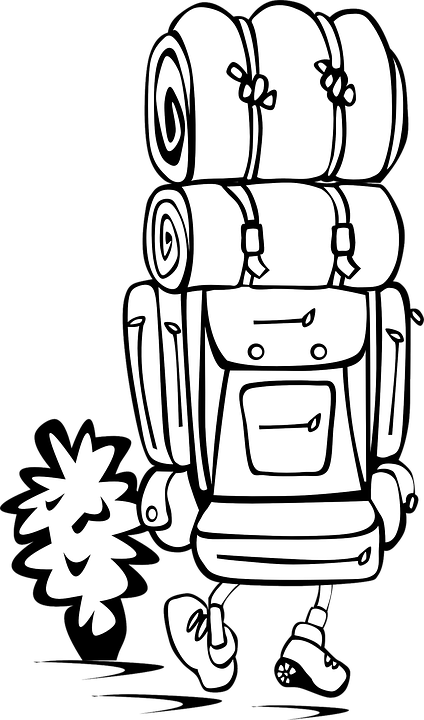
\includegraphics[width=0.3\textwidth]{figures/backpacking.png}\\
		% https://pixabay.com/vectors/backpacking-backpacker-hiking-32069/
	\end{center}
\end{frame}

\begin{frame}
	\frametitle{Lets answer that first question!}

	\begin{problemblock}{Can I get home?}
		Given the current state of the NS rail network, can I get home to Haarlem?
	\end{problemblock}
	\pause
	\begin{answerblock}{Search and ye shall find?}
		We can find out using a Breadth-first or Depth-first search.
	\end{answerblock}
\end{frame}

\begin{frame}
	\frametitle{Depth-first Search}
	\framesubtitle{Recursion rules again}

		\begin{block}{DFS}
			Imagine you are walking in a labyrinth.\\
			\pause
			You bring a some paint and a piece of rope, tie it to the entrance and start walking. Here's what you do:\\
			\pause
			\begin{itemize}
				\item If we come to a cross-way, just pick one direction.
					\pause
				\item If we get to a dead-end, we back up to the last cross-way. Now use the paint to cross out the way you just
					went.
					\pause
				\item Repeat until you find the exit.
			\end{itemize}
		\end{block}	
	
\end{frame}

\begin{frame}
	\frametitle{An implementation}
	
	\begin{algorithmic}
		\Function{DFS}{$v$}
	\pause
		\For{each outgoing edge $e=(v,u)$ of $v$}
	\pause
		\If{$u$ is not visited yet}
		\State mark $u$ as visited
	\pause
		\State\Call{DFS}{$u$}
		\EndIf
		\EndFor
		\EndFunction
		\Comment{Ensure that $v$ is marked as visited before starting}
	\end{algorithmic}
	\pause
	\begin{columns}
		\column{0.455\textwidth}
	\begin{questionblock}{Run time?}
		What is the run time of this algorithm?
		\begin{multicols}{2}
		\begin{enumerate}[A.]
			\item $\Theta(|V|)$
			\item $\Theta(|E|)$
			\item $\Theta(|V| + |E|)$
			\item $\Theta(|V|\times|E|)$
		\end{enumerate}
	\end{multicols}
	\end{questionblock}
		\column{0.455\textwidth}
		\pause
		\begin{answerblock}{}
			Worst-case we consider every vertex once and ever edge once.
		\end{answerblock}
	\end{columns}
\end{frame}

\begin{frame}
	\frametitle{Let's apply it!}

	\begin{problemblock}{Lets draw a graph}
		So lets draw a graph on the smart board and then apply DFS on it!
	\end{problemblock}
\end{frame}

\begin{frame}
	\frametitle{But what if I don't like recursion\dots}
	\framesubtitle{\st{Then tough luck!} Don't worry, we got you covered!}

	\begin{questionblock}{Getting rid of the recursion}
		How could we get rid of the recursion?
		\begin{enumerate}[A.]
			\item Adding nodes to explore to a set and taking the next node to visit randomly from the set.
			\item Adding nodes to explore to a stack and taking the next node to visit from the top of the stack.
			\item Adding nodes to explore to a queue and taking the next node to visit from the front of the queue.
			\item I don't know.
		\end{enumerate}
	\end{questionblock}
\end{frame}

\begin{frame}
	\frametitle{An implementation}
	
	\begin{algorithmic}
		\Function{DFS}{$v$}
		\State $s \gets$ empty Stack
		\State $s$.push($v$)
		\State mark $v$ as visited
		\pause
		\While{$s$ is not empty}
		\State cur $\gets$ $s$.pop()
		\pause
		\For{each outgoing edge $e=(\text{cur},u)$ of $\text{cur}$}
		\If{$u$ is not visited yet}
		\State mark $u$ as visited
		\pause
		\State $s$.push($u$)
		\EndIf
		\EndFor
		\EndWhile
		\EndFunction
	\end{algorithmic}
\end{frame}

\begin{frame}
	\frametitle{So what can we do with this?}

		\begin{exampleblock}{Many use cases!}
			\begin{itemize}
				\item Find a path between vertices, if one exists! (Including finding your way home to Haarlem.)\footnote{Try for
					yourself how you could reconstruct the path from the DFS. Or check page 645 of the book.}
					\pause
				\item Test if $G$ is a connected graph.
					\pause
				\item Find a cycle in $G$ if there is one (that $v$ is a part of).
			\end{itemize}
			
		\end{exampleblock}	
\end{frame}

\begin{frame}
	\frametitle{What if we use a queue though?}
	
	\pause
	\begin{algorithmic}
		\Function{BFS}{$v$}
		\State $s \gets$ empty \alert{Queue}
		\State $s$.enqueue($v$)
		\State mark $v$ as visited
		\While{$s$ is not empty}
		\State cur $\gets$ $s$.dequeue()
		\For{each outgoing edge $e=(\text{cur},u)$ of $\text{cur}$}
		\If{$u$ is not visited yet}
		\State mark $u$ as visited
		\State $s$.enqueue($u$)
		\EndIf
		\EndFor
		\EndWhile
		\EndFunction
	\end{algorithmic}
\end{frame}
	
\begin{frame}
	\frametitle{So what does this BFS do?}

		\begin{block}{BFS}
			We crawl over the graph, layer by layer.\\
			\pause
			First we check all vertices at distance $1$ from our starting point.\\
			\pause
			Then all vertices at distance $2$.\\
			Etc. Etc.
		\end{block}	
	\begin{problemblock}{Lets draw a graph}
		So lets draw a graph on the smart board and then apply BFS on it!
	\end{problemblock}
\pause
	
\end{frame}
